%%%%%%%%%%%%%%%%%%%%%%%%
%
% $Autor: Achal $
% $Datum: 2023-11-24  $
% $Shodrt Description: The foundational concepts and processes involved in deploying Machine Learning for embedded systems. It covers topics from TinyML to anomalies, including data collection, preprocessing, model training, deployment, keyword recognition, feedback, optimization, power management, and handling of outliers. $
% $Directory: ML23-01-Keyword-Spotting-with-an-Arduino-Nano-33-BLE-Sense\report\Contents\en\Domain.tex   $
% $Version: 6.0 $
% $Review by: $
% $Review date: 16.12.2023 $
%
%%%%%%%%%%%%%%%%%%%%%%%%

\chapter{Foundations and Concepts in Machine Learning Deployment for Embedded Systems}
The implementation of TinyML for training datasets on the Arduino Nano BLE Sense 33 to activate the RGB LED in response to valid voice commands involves several critical aspects:

\section{TinyML}
Tiny Machine Learning (TinyML) is a machine learning technique that integrates reduced and optimized machine learning applications that require “full-stack” (hardware, system, software, and applications) solutions. It includes machine learning architectures, techniques, tools, and approaches capable of performing on-device analytics at the very edge of the cloud. TinyML can be implemented in low-energy systems, such as sensors or microcontrollers to perform automated tasks. The technique is still ML, but with less energy and costs and without an internet connection \cite{Ribeiro:2020}.

TinyML introduces Machine Learning to the scene by incorporating Artificial Intelligence into small hardware components. Tiny machine learning is a rapidly growing field of machine learning technologies and applications that includes hardware (dedicated integrated circuits), algorithms, and software capable of performing on-device sensor data analytics at extremely low power.

In summary, the application of TinyML for training datasets on the Arduino Nano BLE Sense 33 to blink its RGB LED in response to valid voice commands involves a combination of hardware, software, and machine learning techniques, tailored to the device's constraints and requirements. This technology enables voice-controlled interactions in embedded systems, making it suitable for a variety of applications, from home automation to assistive devices\cite{Mishra:2023}.

\section{Data Collection}
To train a TinyML model for voice command recognition, a dataset of audio samples containing both the target keywords and background noise should be collected. These samples are recorded using the onboard microphone of the Arduino Nano BLE Sense 33.


\section{Data Preprocessing}
Data preprocessing involves converting the raw audio data into a suitable format for model training. This may include feature extraction, such as MFCC (Mel-frequency cepstral coefficients), to represent the audio in a way that is amenable to machine learning. Please refer to Figure \ref{fig:DataPreprocessingFlow}

\begin{figure}[h!]
	\centering
	%%%%%%%%%%%%%%%%%%%%%%%%
%
% $Author: Achal Shakywar $
% $Datum: 15.12.2023  $
% $Pfad: MLProject\ML23-01-Keyword-Spotting-with-an-Arduino-Nano-33-BLE-Sense\report\Images\Domain\DataPreprocessingFlow.tex$
% $Version: 1.0 $
%
% !TeX encoding = utf8
%
%%%%%%%%%%%%%%%%%%%%%%%%

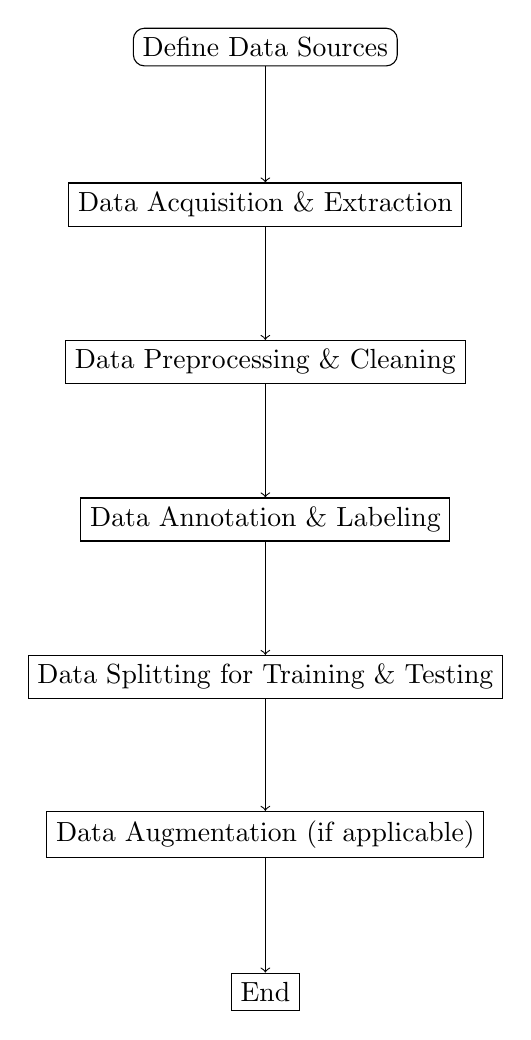
\begin{tikzpicture}[node distance=2cm, auto]
    % Nodes
    \node (sources) [draw, rounded corners] {Define Data Sources};
    \node (acquisition) [draw, below of=sources] {Data Acquisition \& Extraction};
    \node (preprocessing) [draw, below of=acquisition] {Data Preprocessing \& Cleaning};
    \node (annotation) [draw, below of=preprocessing] {Data Annotation \& Labeling};
    \node (splitting) [draw, below of=annotation] {Data Splitting for Training \& Testing};
    \node (augmentation) [draw, below of=splitting] {Data Augmentation (if applicable)};
    \node (end) [draw, below of=augmentation] {End};

    % Arrows
    \draw [->] (sources) -- (acquisition);
    \draw [->] (acquisition) -- (preprocessing);
    \draw [->] (preprocessing) -- (annotation);
    \draw [->] (annotation) -- (splitting);
    \draw [->] (splitting) -- (augmentation);
    \draw [->] (augmentation) -- (end);

\end{tikzpicture}


	\caption{Flow of Data Preprocessing} \label{fig:DataPreprocessingFlow}
\end{figure}

\section{Model Training}
The collected and preprocessed audio data is used to train a TinyML model. Training may involve techniques like transfer learning, quantization, and model compression to ensure the model's size and computational requirements are compatible with the Arduino Nano BLE Sense 33's limitations. See Figure \ref{fig:ModelTrainingFlow}

\begin{figure}[h!]
	\centering
	%%%%%%%%%%%%%%%%%%%%%%%%
%
% $Author: Achal Shakywar $
% $Datum: 15.12.2023  $
% $Pfad: MLProject\ML23-01-Keyword-Spotting-with-an-Arduino-Nano-33-BLE-Sense\report\Images\Domain\ModelTrainingFlow.tex$
% $Version: 1.0 $
%
% !TeX encoding = utf8
%
%%%%%%%%%%%%%%%%%%%%%%%%

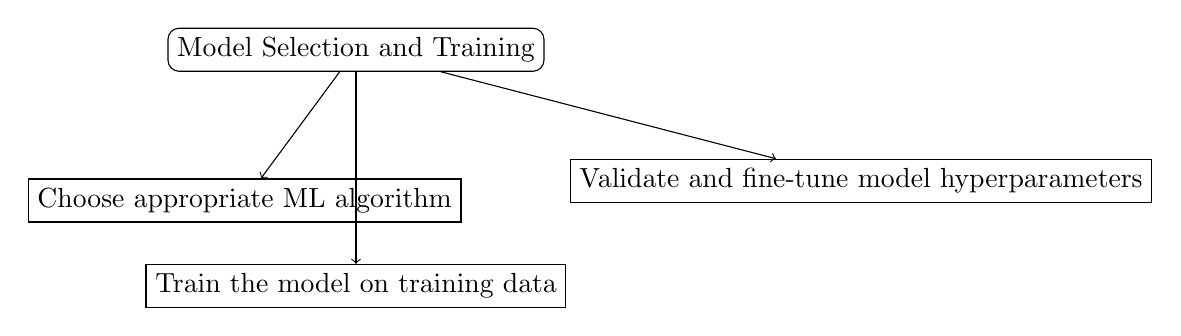
\begin{tikzpicture}[node distance=2cm, auto]
	% Nodes
	\node (model) [draw, rounded corners] {Model Selection and Training};
	\node (algo) [draw, below left of=model, xshift=-0cm, yshift=-0.5cm] {Choose appropriate ML algorithm};
	\node (train) [draw, below of=model, yshift=-1cm] {Train the model on training data};
	\node (validate) [draw, below right of=model, xshift=5cm, yshift=-0.25cm] {Validate and fine-tune model hyperparameters};
	
	% Arrows
	\draw [->] (model) -- (algo);
	\draw [->] (model) -- (train);
	\draw [->] (model) -- (validate);
	
\end{tikzpicture}

	\caption{Flow of Model Training} \label{fig:ModelTrainingFlow}
\end{figure}

\section{Model Deployment}
Once the TinyML model is trained, it is deployed onto the Arduino Nano BLE Sense 33. The model must be integrated into the device's firmware and take advantage of the available software libraries for inference. See Figure \ref{fig:ModelDeployment}

\begin{figure}[h!]
	\centering
	%%%%%%%%%%%%%%%%%%%%%%%%
%
% $Author: Achal Shakywar $
% $Datum: 15.12.2023  $
% $Pfad: MLProject\ML23-01-Keyword-Spotting-with-an-Arduino-Nano-33-BLE-Sense\report\Images\Domain\ModelDeployment.tex$
% $Version: 1.0 $
%
% !TeX encoding = utf8
%
%%%%%%%%%%%%%%%%%%%%%%%%

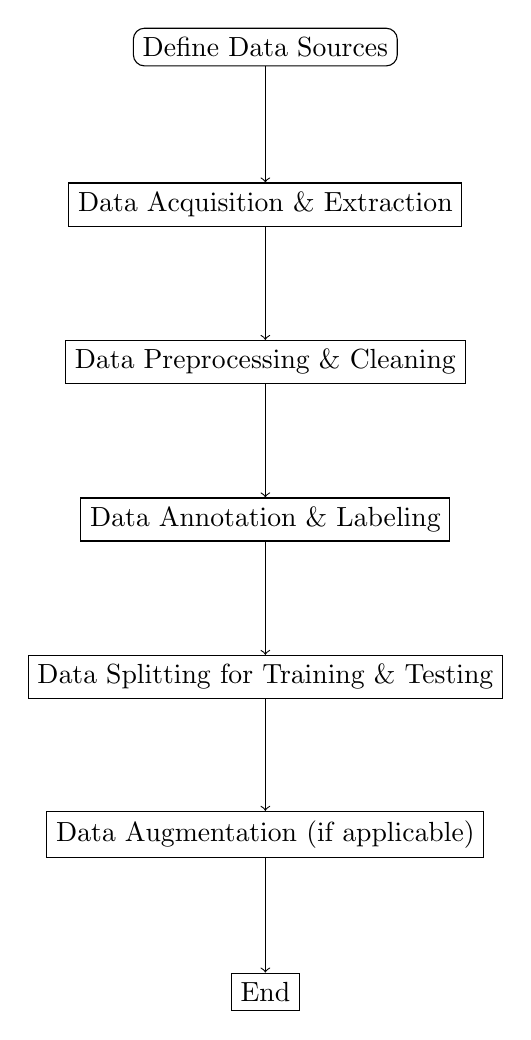
\begin{tikzpicture}[node distance=2cm, auto]
	% Nodes
	\node (sources) [draw, rounded corners] {Define Data Sources};
	\node (acquisition) [draw, below of=sources] {Data Acquisition \& Extraction};
	\node (preprocessing) [draw, below of=acquisition] {Data Preprocessing \& Cleaning};
	\node (annotation) [draw, below of=preprocessing] {Data Annotation \& Labeling};
	\node (splitting) [draw, below of=annotation] {Data Splitting for Training \& Testing};
	\node (augmentation) [draw, below of=splitting] {Data Augmentation (if applicable)};
	\node (end) [draw, below of=augmentation] {End};
	
	% Arrows
	\draw [->] (sources) -- (acquisition);
	\draw [->] (acquisition) -- (preprocessing);
	\draw [->] (preprocessing) -- (annotation);
	\draw [->] (annotation) -- (splitting);
	\draw [->] (splitting) -- (augmentation);
	\draw [->] (augmentation) -- (end);
	
\end{tikzpicture}

	\caption{Block Diagram for Model Deployment } \label{fig:ModelDeployment}
\end{figure}

\section{Keyword Recognition}
In the deployed system, the TinyML model continuously analyzes audio data from the onboard microphone to recognize specific keywords or commands. When a valid keyword is detected, a response is triggered to blink the RGB LED on the Arduino Nano BLE Sense 33.

\section{Feedback and Optimization}
Continuous monitoring and feedback are essential for improving the recognition performance. Optimization may include fine-tuning the model, enhancing noise filtering, and refining the response mechanism to ensure accurate and reliable keyword recognition.

\section{Power Management}
Since the Arduino Nano BLE Sense 33 runs on a limited power source, power management is a critical consideration. Implementing low-power modes and strategies to minimize energy consumption is essential for prolonged operation.

\section{Outliers}
In Machine Learning, an \textbf{outlier} is a data point that deviates significantly from the rest of the dataset. They are often abnormal observations that skew the data distribution, and arise due to inconsistent data entry, or erroneous observations. Outliers can skew and mislead the training process of machine learning algorithms resulting in longer training times, less accurate models, and ultimately poorer results \cite{Nichani:2020}.

Outliers can be detected using various techniques such as:
\begin{enumerate}
	\item \textbf{Standard Deviation:} When the data, or certain features in the dataset, follow a normal distribution, you can use the standard deviation of the data, or the equivalent z-score to detect outliers \cite{C:2022}.
	
	\item \textbf{Clustering based outlier detection:} In the K-Means clustering technique, each cluster has a mean value. Objects belong to the cluster whose mean value is closest to it. In order to identify the Outlier, firstly we need to initialize the threshold value such that any distance of any data point greater than it from its nearest cluster identifies it as an outlier for our purpose.
\end{enumerate}

In the context of \textbf{speech recognition}, outliers can be particularly challenging. For example, a segment-based speech recognizer built on a neural net has to identify outliers as well. One approach is to artificially generate outlier samples, but this is tedious, error-prone, and significantly increases the training time. An alternative is applying a replicator neural net for this task, originally proposed for outlier modeling in data mining. This approach allows the recognizer to perform similarly without the need for a large amount of outlier data.

Please note that dealing with outliers often requires domain expertise, and none of the outlier detection techniques should be applied without understanding the data distribution and the use case. 

\section{Anomalies}
In Machine Learning, \textbf{anomalies} are data points that stand out from other data points in the dataset and don’t confirm the normal behavior in the data\cite{Kumar:2023}. These data points or observations deviate from the dataset’s normal behavioral patterns\cite{Johnson:2023}. Anomaly detection is an unsupervised data processing technique to detect anomalies from the dataset.

Anomaly detection plays an instrumental role in robust distributed software systems. It can enhance communication around system behavior, improve root cause analysis, reduce threats to the software ecosystem, and is commonly used for data cleaning, intrusion detection, fraud detection, systems health monitoring, event detection in sensor networks, and ecosystem disturbances.

In the context of \textbf{speech recognition}, anomalous audio in speech recordings is often caused by speaker voice distortion, external noise, or even electrical interferences. These obstacles have become a serious problem in some fields, such as high-quality dubbing and speech processing. A novel approach using a temporal convolutional attention network (TCAN) is proposed to tackle this problem. The use of temporal conventional network (TCN) can capture long-range patterns using a hierarchy of temporal convolutional filters. To enhance the ability to tackle audio anomalies in different acoustic conditions, an attention mechanism is used in TCN, where a self-attention block is added after each temporal convolutional layer\cite{Huang:2021}. This aims to highlight the target-related features and mitigate the interferences from irrelevant information.



